\vspace{10pt}

{\centering\subsection*{韩念秋:我的乐园}}

\addcontentsline{toc}{subsection}{韩念秋:我的乐园}

\renewcommand{\leftmark}{韩念秋:我的乐园}

\begin{figure}[htbp]

\centering

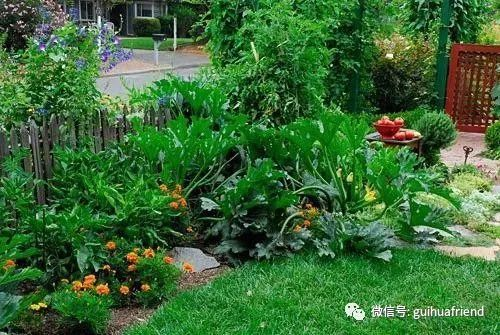
\includegraphics[width = .5\textwidth]{./ch/41.jpg}

\end{figure}



推开大门。只闻到一阵瓜果飘香,又见一片万紫千红,这就是我外公家的前院,我外公家的前院十分宽敞,半个院子都种满了蔬菜。夏天到了,我经常去村子里的小卖部买几根雪糕,走在小路上吃,周围是那么的安静,就连蝉热的也不叫了。一到家,我总能目睹一场别有风趣的音乐会,红红的辣椒歪歪扭扭的站成一排,唱着那火辣辣的歌;蜜蜂在微风中有节奏地跳舞,这时蝉终于出现了,它与麻雀一起来告诉我这个乐园的美妙。我装成受邀的成员也急忙的赶了过去。抓起了一只蝉的翅膀,想让她带我一起飞到天上。飞呀飞,飞呀飞,可我却始终飞不起来,我准备放弃的时候,转念一想,立刻扑到了鸟儿跟前,我手一伸,它一躲,我手又一伸,它又一躲,我心想它怎么比我还敏捷?这个小院是我心中永远的乐园,再无其二。



\vspace{10pt}



作者:四(1)班 韩念秋

指导老师:周瑞

投稿:2021年4月15日

发表:2021年4月21日


                



\vspace{10pt}

\hline



